\documentclass[letterpaper,11pt]{article}
\usepackage{etex}
\usepackage{enumitem}
\reserveinserts{28}
\usepackage{amssymb}
\usepackage{theorem}
%\usepackage{savetrees}
\usepackage[margin=2cm]{geometry}
\usepackage{graphicx}
\usepackage{fancybox}
\usepackage{fancyhdr}
\usepackage{tabularx}
\usepackage{color}
\usepackage{xcolor}
\usepackage{multirow}
\usepackage{amsmath}
\usepackage[utf8]{inputenc} % Pour pouvoir taper les accent directement et non pas passer par \'
\usepackage[T1]{fontenc} %%% Pour que les accents soient correctement traités dans le PDF et le DVI
\usepackage{lmodern} %Un autre package pour les accents français
\usepackage[french]{babel} %Un autre package pour les accents
\usepackage{ifthen}
%\usepackage{multicol}
%\usepackage{cancel}
\usepackage{pst-all}
\usepackage{pstricks-add}
\usepackage{multicol}
%\usepackage{tikz}
%\usepackage{pgf,tikz}
%\usepackage{circuitikz}
%\usetikzlibrary{shapes}
%\usetikzlibrary{calc}
%\usetikzlibrary{plotmarks}
%\usepackage{tkz-fct}
\usepackage{fp}
\usepackage{float}
\usepackage{siunitx}
\usepackage{pdfpages}%Pour sortir seulement certaine pages du pdf
\usepackage{textcomp}
\usepackage{hyperref}
\hypersetup{
    colorlinks=true, % make the links colored
    linkcolor=blue, % color TOC links in blue
    urlcolor=red, % color URLs in red
    linktoc=all % 'all' will create links for everything in the TOC
}

\sisetup{locale = FR, number-math-rm, per-mode=symbol, separate-uncertainty}

\renewcommand{\exp}[1]{\mathrm{e}^{#1}}

\setlength{\parindent}{0pt}



\begin{document}


\begin{center}
~
\vfill
\LARGE{Travail Pratique 2 (IFT-4201/IFT-7201)}\\[0.4cm]

\Large{Présenté à Audrey Durand}

\vfill
\large{Équipe 10: Adam Cohen, Maxime Genest, Vincent Masse}

\vfill
\thispagestyle{empty}

\end{center}

\clearpage

\pagestyle{fancy}
\lhead{IFT-7201}
\chead{Devoir 2 (Automne 2020)}
\rhead{Équipe 10}

\textbf{Remarque concernant le code:}\\

Pour le numéro 1, le notebook <<test\_no\_1.ipynb>> doit être utilisé pour produire les résultats (il suffit de compiler toutes les cellules dans l'ordre). À noter que la façon dont les germes aléatoires étaient fixés dans le fichier de départ fourni ne semble pas fonctionné entièrement, de sorte qu'en compilant le notebook, il se peut que vous obteniez des résultats un peu différent, mais similaires à ceux présentés.\\

Pour le numéro 2, le fichier q2.py (qui appelle tilecoding.py) doit être exécuté.

\clearpage

\section{Deep $Q$-learning}

\begin{enumerate}[label=(\alph*)]

\item \textbf{État comme seule entrée}\\
La fonction prenant en entrée seulement l'état permet d'avoir plus de flexibilités.
Avec cette fonction, il est possible d'avoir des poids différents pour chaque action, ce qui n'est pas possible avec la fonction qui prend en entrée (état-action). En effet, avec la fonction état-action, on peut seulement ajouter des paramètres qui modifiera la sortie pour la valeur Q, alors que pour la fonction qui prend seulement l'état en entrée, on a des poids différent pour chaque action.

\item \textbf{Réseau cible}\\
L'oubli catastrophique est le fait qu'un réseau de neurones oubli son apprentissage en changeant d'avis trop rapidement en se basant sur des observations récentes. Le fait de fixer les poids $\theta$ dans la cible pendant plusieurs mise à jours permet de conserver une certaine stabilité pour permettre la convergence. Lors de la période pour laquelle la cible inchangée, le réseau peut observer des mauvaises récompenses associées à une action et continuer à l'exploiter car les poids ne seront pas mis à jour. Sinon, il modifierait trop rapidement les poids, ce qui causerait trop de variance dans le choix des actions. Le fait de fixer la cible permet de ne pas désapprendre après une certaine observation menant à des mauvaises récompenses.  

\item \textbf{Heuristique}\\
Si $\tau$ est trop grand, la cible est trop modifiée, ce qui risque de compromettre la convergence (voir numéro précédent), le cas limite $\tau=1$ revient à ne pas fixer (même pas partiellement) les cibles. Si $\tau$ est trop petit, les cibles seront trop fixes, et donc les cibles ne sont pratiquement pas améliorées et le réseau apprend donc sur des moins bonnes cibles (non-représentative de ce que l'on doit viser). Le cas limite $\tau=0$ montre un cas où la cible n'est jamais modifiée et gardera toujours sa valeur initiale, ce qui est bien entendu non-souhaitable. 

\item \textbf{Replay buffer}\\
L'avantage de son utilisation est de briser la corrélation entre les échantillons utilisés lors de la mise à jour (le tuple $(s_t, a_t, r_{t+1}, s_{t+1})$ et le tuple suivant $(s_{t+1}, a_{t+1}, r_{t+2}, s_{t+2})$ partage le même état $s_{t+1}$). Cela compromet l'apprentissage. Le fait de stocker les échantillons et d'échantillonner une mini-batch aléatoire à chaque pas de temps permet de contourner ce problème. 

\item \textbf{Apprentissage supervisé}\\
La distribution $\mathcal{D}$ du replay Buffer réfère à un échantillonnage dans une banque de données qui a été créée par l'agent lui-même, ce dernier est responsable de créé son propre <<dataset>>. Alors qu'en apprentissage supervisé (pour faire de la régression notamment), le jeux de données d'apprentissage n'est pas établi par l'agent, il lui est fourni (ou du moins la loi de probabilité qui détermine ces données n'est pas influencée par les décisions d'un agent).

\item Parmi les défis d'implémentation auxquels on a fait face, l'un d'entre eux et la longueur d'un entraînement, cela a fait en sorte qu'il était difficile de tester différents paramètres d'entraînements et d'optimiser cette dernières. Une ressource de calcul plus puissante que nos ordinateurs personnels aurait sans doute permis de faire un plus large éventail de tests. De plus, après avoir simuler plusieurs entraînements sans varier les paramètres et le critère d'arrêt, on observe que le nombre de trajectoires à faire avant la convergence est très variable et semble beaucoup sujet à l'aléatoire. Nous avons l'impression que si l'agent est chanceux dans ces trajectoires et qu'il touche à un moment donné un gain substantiel, à partir de ce moment sa courbe d'apprentissage change abrutement et il enligne plusieurs séquences de trajectoires succès. Nous avons simulé plusieurs apprentissages avec le critère d'arrêt suivant: Avoir une moyenne de gain de plus de 200 dans les 5 dernières trajectoires effectuées. Avec ce critère d'arrêt, la méthode convergeait parfois en 400 trajectoires, parfois en 1600 trajectoires. Aussi, nous avons observé un comportement particulier sur certaines simulations: À l'occasion, l'apprentissage semblait près d'obtenir le critère d'arrêt, mais se mettait à replonger vers des gains négatifs pour une très longue séquence avant de remonter vers des gains importants. Il n'est pas à écarter l'hypothèse que cela serait en fait de l'oubli <<catastrophique>> en lien avec une valeur de $\tau$ non-optimale. Finalement, en optant pour un paramètre <<epsilon\_decay>> de 0.95, nous avons observé une convergence plus rapide (mais restant très variable).\\

Voici deux graphiques illustrant l'évolution des gains épisodiques ainsi que l'évolution de la fonction de perte durant un entraînement.

\begin{center}
\begin{figure}[H]
\caption{Évolution des gains et fonction de pertes sur une courbe d'apprentissage <<rapide>>}\label{figure rapide}
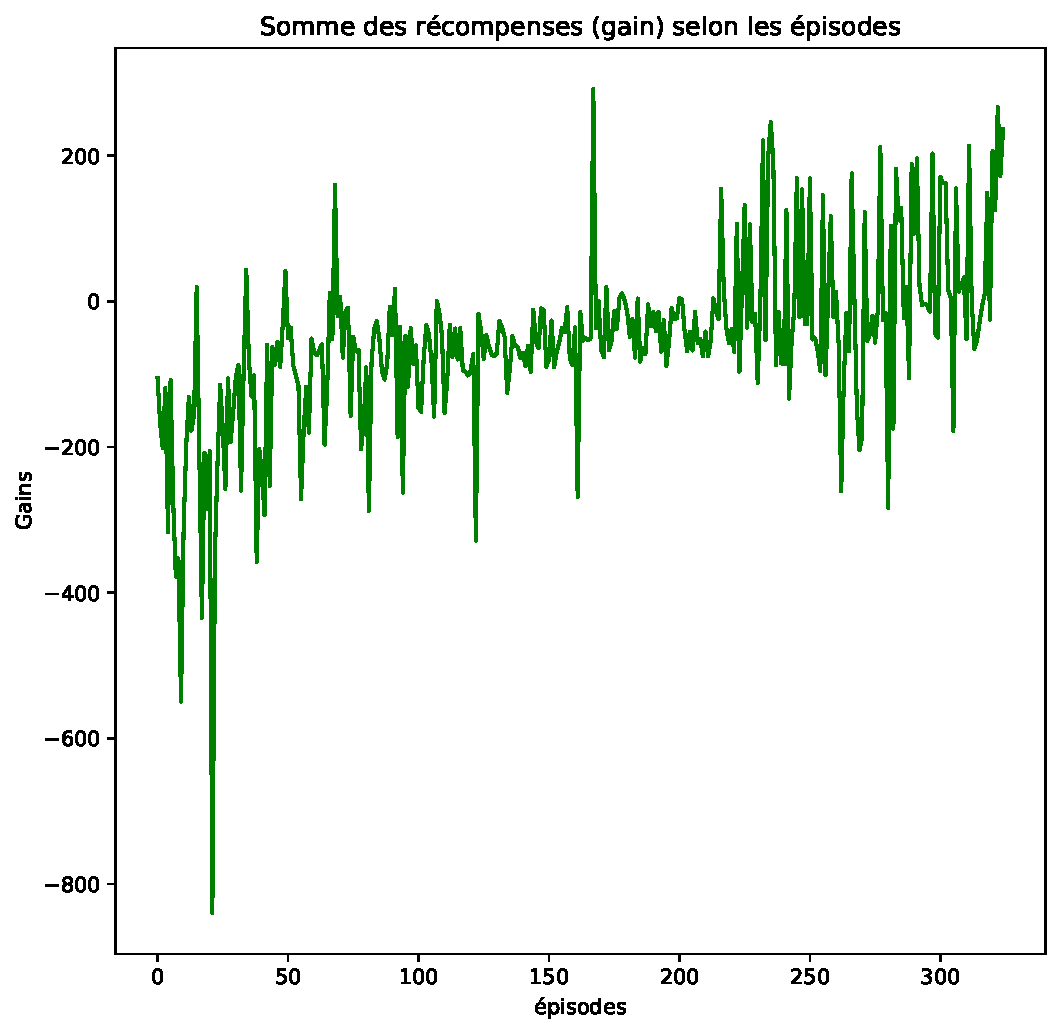
\includegraphics[width=0.45\linewidth]{gains_convergence_rapide.pdf} \hfill 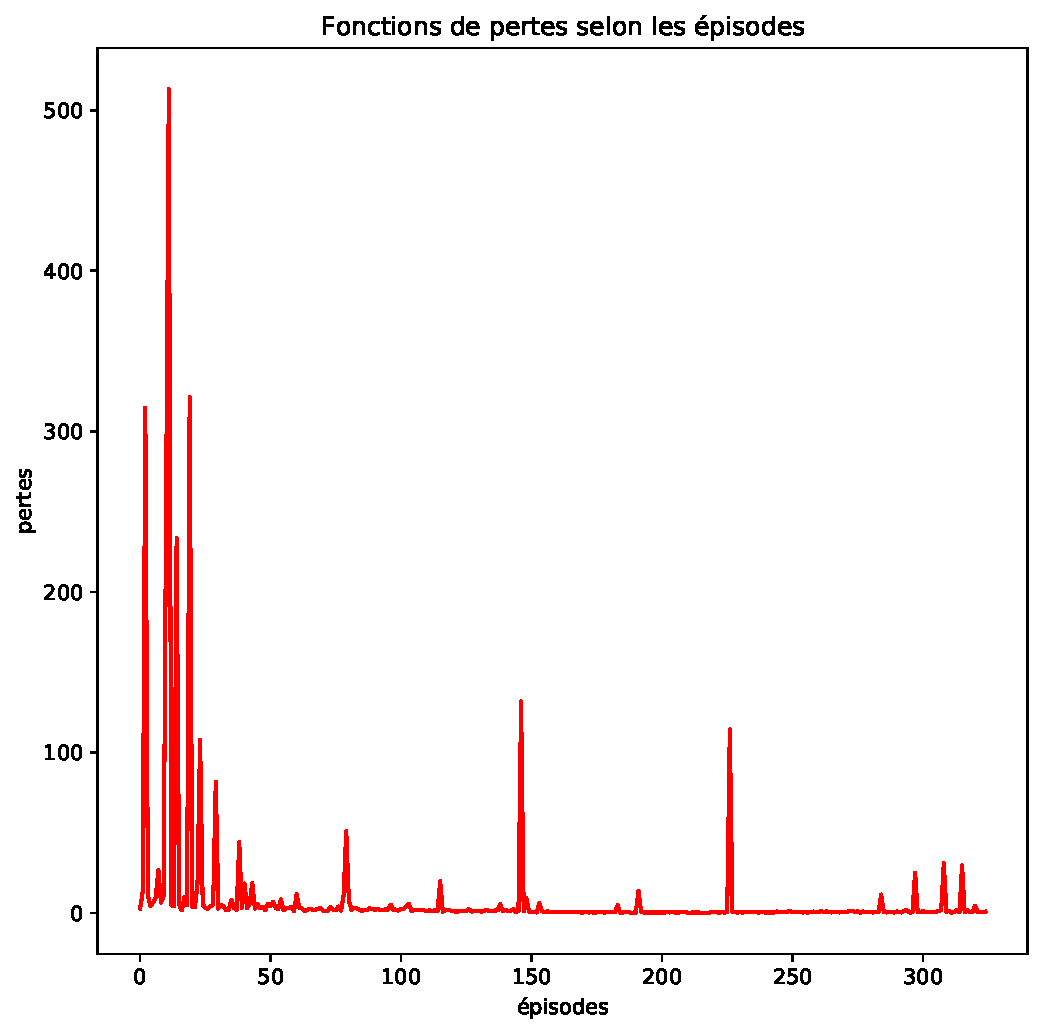
\includegraphics[width=0.45\linewidth]{pertes_convergence_rapide.pdf}
\end{figure}
\end{center}

\vspace*{-1.5cm}
Voici maintenant un graphique de la fonction de gain par pas de temps dans l'environnement pour un épisode joué par notre agent entraîner (donc par la politique apprise) ainsi que le graphique des gains cumulés pour ce même épisode.
 
\begin{figure}[H]
\begin{center}
\caption{Gains instantanés et cumulé durant un épisode}
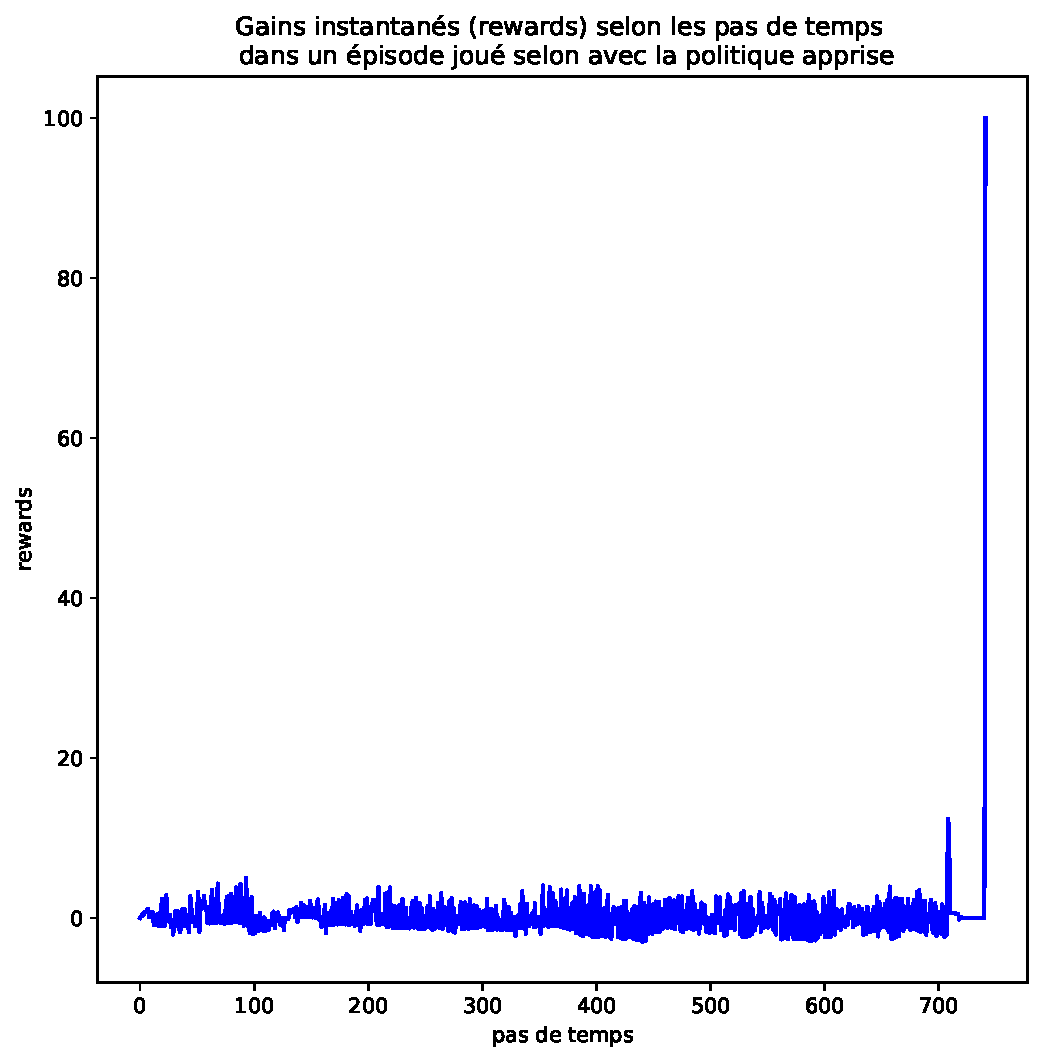
\includegraphics[scale=0.45]{gain_par_pas_apres_cv.pdf}\hfill 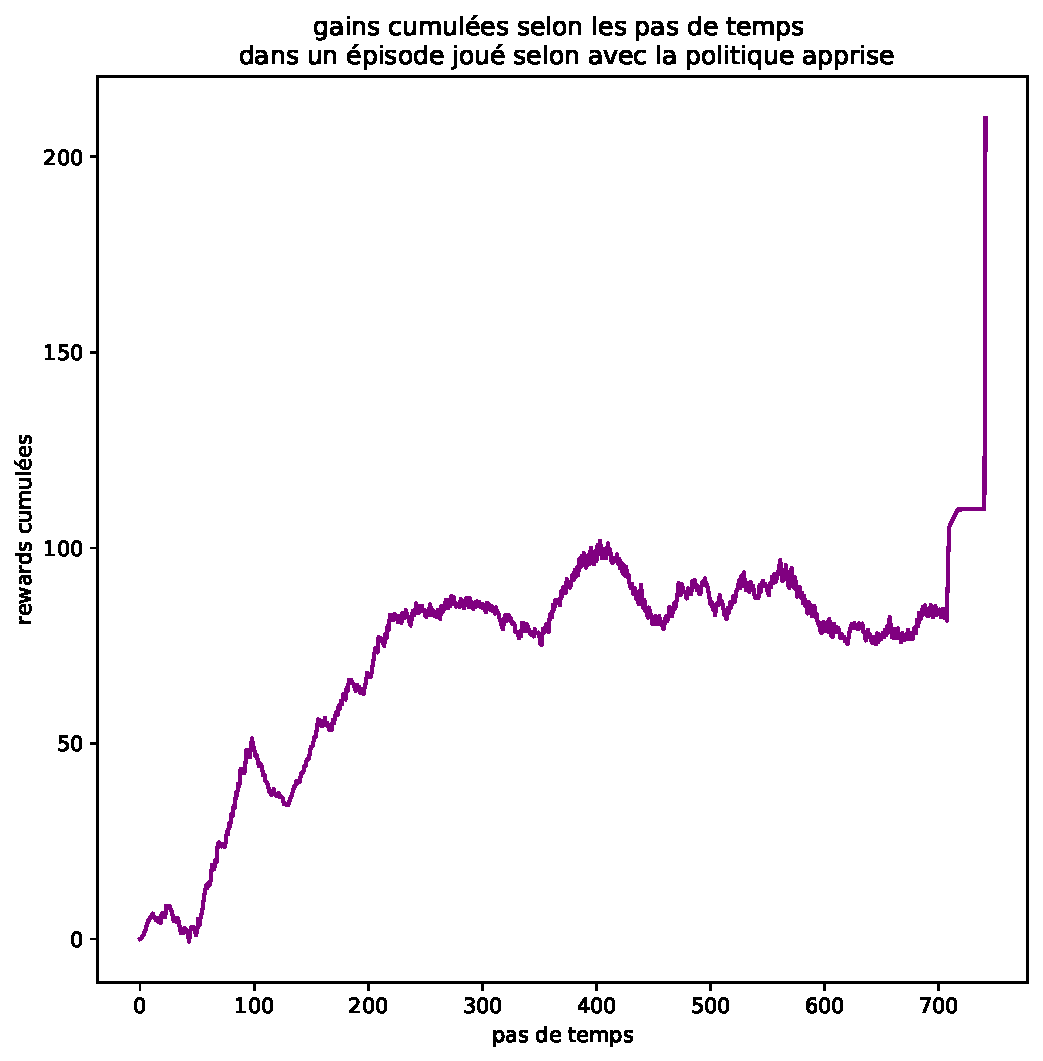
\includegraphics[scale=0.45]{gains_cumules_par_pas_apres_cv.pdf}
\end{center}
\end{figure}

\end{enumerate}

\section{SARSA($\lambda$)}

\begin{enumerate}[label=(\alph*)]

\item \textbf{Exploration}\\
L'initialisation de la fonction de valeurs d'actions est associée à l'initialisation des estimateurs empiriques des actions dans l'approche des bandits. Dans cet environnement, puisque l'on initialise les $Q(s,a)=0$ et que la fonction de reward donne un reward de $-1$ à toutes les actions ou l'auto n'atteint pas le drapeau, cela revient à faire une initialisation optimiste de l'estimateur. En effet, en initialisant tous les $Q_{vals}=0,$ toutes les actions essayées feront pire que les actions dont la valeur est encore la valeur initiale, ainsi cela force l'algorithme à essayer les autres actions possibles.

\item \textbf{Implementation}\\
Nous avons implémenté l'algorithme SARSA$(\lambda)$ avec caractéristiques binaires. La particularité était l'espace joint des états et des actions représentés par un quadrillage.
Nous avons ensuite fait plusieurs simulations sur l'environement \textit{MountainCarV0} de openAI gym.
Pour chaque simulation, nous avons entrainé le modèle sur 500 épisodes d'au plus de 200 pas de temps.\\

SARSA$(\lambda)$ nous permet d'introduire l'idée de <<trace d'éligibilité>>, celle-ci va agir sur la propagation de la différence temporel $\delta$ pour notamment les états <<éligibles>>, c'est-à-dire ceux visités récemment.
$\lambda$ lui, agit directement sur cette trace d'éligibilité, il peut donc donner plus ou moins d'importance aux états visités récemment en contrôlant leurs déclins dans le temps sachant qu'au départ, ils sont fixés à 1.
La trace d'éligibilité entre en jeu lors de la maximisation des poids $\Theta$.
\begin{eqnarray*}
Q(s,a) & = & Q(s,a) + \alpha \delta e(s,a) \\
e(s,a) & \leftarrow &  \gamma \lambda e(s,a)
\end{eqnarray*}
Nous avons fait des simulations pour les valeurs, 0, 0.5, 0.9 et 1 de $\lambda$. On peut tout d'abord noter que pour tout $\lambda \geq$ 1, la somme des gains par épisodes est constante, cela se résume par l'importance des états qui ne décroissent pas dans le temps, l'agent ne peut donc pas explorer convenablement surtout au début de chaque épisode. Le graphique suivant présente la moyenne mobile des 100 derniers\footnote{Au début, lorsqu'il y a moins de 100 épisodes de joués, ça correspond seulement à la moyenne.} gains épisodiques 
\begin{figure}[H]
\label{figure: variance petite}
\caption{Evolution de la moyenne des 100 derniers gains épisodiques}
\begin{center}
\includegraphics[scale=0.45]{SARSA_lambda_gains.png}
\end{center}
\end{figure}
Pour $\lambda$ = 0, on assume de ne pas prendre en compte la trace d'éligibilité dans la maximisation des poids $\Theta$, c'est donc équivalant à un algorithme SARSA.\\

On doit donc avoir $0 < \lambda < 1$ pour qu'il ait un véritable impact sur l'apprentissage.
Pour les deux dernières simulations, nous avons fait des expériences sur une valeur équilibré de $\lambda$ et une valeur se rapprochant de 1.
Dans le cas de $\lambda$ = 0.9 où les états rencontrés vont avoir plus d'importance sur le temps, on observe une baisse des gains à peu près à partir du $140^{\text{ième}}$ épisode, contrairement au cas où $\lambda$ est à 0.5, la courbe est plus linéaire sur le temps, de plus on observe qu'entre les épisodes 140 et 280, les gains sont plus élevés pour 0.5 on peut donc dire que pour un nombre d'épisodes plus limité il serait préférable d'opter pour une valeur de $\lambda$ plus faible. Le paramètre 0.9 reste globalement plus performant que la simulation où $\lambda = 0.5,$ surtout dans la perspective de l'atteinte d'une moyenne de gains sur 100 épisodes de plus de $-110,$ ce critère est rencontré dans le cas $\lambda=0.9$ seulement. 

\end{enumerate}

\end{document}
